\section{Experiments}

\subsection{Experimental Setup}
\textbf{Models and Benchmarks} We implement our method on two representative dLLMs, Llada-1.5 and Dream-7B-Instuct, to evaluate its effectiveness in accelerating the inference process across various tasks. We conduct experiments on four standard benchmarks covering diverse task types to ensure the broad applicability of our approach, including GSM8K (mathematical reasoning), MATH(mathematical problem solving), HumanEval (code generation), and Ruler (long context capability).   

\textbf{Baselines and Metrics}
To validate the effectiveness of our method, we compare Step-dLLM against several state-of-the-art dLLM-based approaches, including vanilla LLaDA and Dream, the sparse acceleration method for autoregressive models StreamingLLM, and training-free efficient dLLM methods such as Fast-dLLM and SparseD. We evaluate inference acceleration and generation quality using quantitative metrics. Inference speed is quantified by the wall-clock time required to complete each task under a fixed generation length, while generation quality is assessed using task-specific metrics, such as accuracy on GSM8K, to reflect model performance under different acceleration strategies.

\textbf{Implemention Details}
During inference, we use a single NVIDIA H100 GPU and fix the batch size to 1 for all models. In our proposed method Step-dLLM, we largely follow the hyperparameter settings of SparseD. Specifically, for all datasets, we set the granularity of sparsity computation (block size) to \(S = 16\) and the block length to \(L = 32\), which controls the proportion between autoregressive steps and diffusion steps. In addition, we set the refresh frequency of the attention mask matrix to 0.2, i.e., we update the global attention mask every \(0.2 \times N_{\text{steps}}\) denoising steps. For short-text datasets such as GSM8K and HumanEval, we set the sparsity budget to \(\rho = 50\%\), whereas for the long context dataset Ruler, we adopt a more conservative budget of \(\rho = 20\%\). We use the same configuration \((S, L, \rho)\) for SparseD. Regarding the parameter in SparseD that controls the use of full attention instead of sparse attention in the early steps, we set the proportion to \(\text{skip}\% = 5\%\). To ensure a fair comparison, we configure Fast-dLLM with the same block length \(L = 32\) and set the threshold to \(\text{threshold} = 0.9\). For StreamingLLM, we fix the proportion of sink tokens \(s_0\) to 10\% of the total generation length, and derive the sliding window size \(W\) from the sparsity budget as $W = (\rho - s_0) \cdot L_{\text{total}}.$
Across all methods, we set the total generation length \(L_{\text{total}}\) to be equal to the number of diffusion steps \(N_{\text{steps}}\). Additional details about the models, datasets, and baseline methods are provided in the Appendix.

\subsection{Main Results}

Tables~\ref{tab:main-bs16-llada} and~\ref{tab:main-bs16-dream} summarize the main comparison on LLaDA-1.5 and Dream-7B-Instruct. Overall, Step-dLLM provides the best accuracy--sparsity trade-off among sparse methods on both short-form and long-context benchmarks, and the advantage becomes more visible as sparsity increases.

On reasoning and code generation tasks, Step-dLLM stays close to dense decoding at moderate sparsity and degrades more gracefully than SparseD in the high-sparsity regime. At 50\% sparsity, its accuracy is already comparable to the dense baseline on both backbones. The difference becomes clearer at 90\% sparsity: on GSM8K, Step-dLLM improves over SparseD by 5.6 points on LLaDA-1.5 (35.25\% vs.\ 29.64\%) and by 10.5 points on Dream-7B-Instruct (32.68\% vs.\ 22.21\%). At 95\% sparsity, the gap further widens on GSM8K, where Step-dLLM retains 17.13\% and 15.31\% accuracy on the two models, compared with 9.86\% and 4.40\% for SparseD. Similar trends hold on MATH and HumanEval. This behavior is consistent with our core hypothesis: once denoising progresses, a mask computed only once becomes increasingly stale, while periodic refresh better matches the evolving attention structure.

The gains are even larger on long-context retrieval benchmarks. On NIAH and RULER, Step-dLLM remains much closer to dense performance on the harder multi-needle and compositional subtasks, where missing a small set of relevant positions can lead to a disproportionate accuracy drop. For example, on LLaDA-1.5 at 80\% sparsity, SparseD drops to 71.20\% on NIAH-S\_3 and 74.20\% on MK\_3, whereas Step-dLLM maintains 100.00\% and 99.60\%, respectively. A similar trend appears on Dream-7B-Instruct, where Step-dLLM improves over SparseD by 21.8 points on S\_3 and 18.6 points on MK\_3 at the same sparsity level. On RULER, Step-dLLM also yields clear gains on compositional tasks such as CWE, improving LLaDA-1.5 from 34.56\% to 54.16\% at 90\% sparsity. These results suggest that long-context generation is especially sensitive to stale sparse patterns, because the set of salient key positions can shift substantially across denoising steps.

In contrast, StreamingLLM performs poorly throughout and often collapses at high sparsity. On LLaDA-1.5, GSM8K drops from 74.07\% at 50\% sparsity to 19.11\% at 80\% sparsity and essentially zero at 90\%; Dream-7B-Instruct shows the same failure mode. This result is expected: StreamingLLM is designed for autoregressive causal attention, whereas diffusion LLMs rely on bidirectional interactions that evolve during denoising. The comparison therefore highlights that sparse patterns tailored for autoregressive decoding do not transfer directly to the diffusion setting.

\begin{table}[t]
\centering
\caption{Main results on LLaDA-1.5 with block size 16. All values are accuracy (\%). \textbf{Bold} marks the best result per sparsity level (excluding Dense).}
\label{tab:main-bs16-llada}
\setlength{\tabcolsep}{3.5pt}
\renewcommand{\arraystretch}{1.15}

\resizebox{\textwidth}{!}{%
\begin{tabular}{@{}ll ccc ccccccccc ccccc@{}}
\toprule
\multirow{2.5}{*}{\textbf{Method}} & \multirow{2.5}{*}{\textbf{Sparsity}}
  & \multicolumn{3}{c}{\textbf{Short-form}}
  & \multicolumn{8}{c}{\textbf{NIAH}}
  & \multicolumn{5}{c}{\textbf{RULER}} \\
\cmidrule(lr){3-5} \cmidrule(lr){6-13} \cmidrule(l){14-18}
& & GSM8K & Math & HumanE
  & $\text{S}_1$ & $\text{S}_2$ & $\text{S}_3$
  & $\text{MK}_1$ & $\text{MK}_2$ & $\text{MK}_3$
  & MQ & MV
  & VT & CWE & FWE & QS & QH \\
\midrule

Dense & --
  & \textbf{81.04} & \textbf{37.20} & \textbf{40.24}
  & \textbf{100.0} & \textbf{100.0} & \textbf{100.0} & \textbf{100.0}
  & \textbf{100.0} & \textbf{100.0} & \textbf{100.0} & \textbf{100.0}
  & \textbf{100.0} & \textbf{52.40} & \textbf{64.20} & \textbf{91.30} & \textbf{76.00} \\

\midrule
\multirow{3}{*}{StreamingLLM}
  & 50\% & 74.07 & \textbf{38.20} & 39.02
    & 20.80 & 20.20 & 18.40 & 21.20 & 20.40 & 15.40 & 19.20 & 14.40
    & 30.60 & 13.40 & 73.80 & 81.65 & 44.40 \\
  & 80\% & 19.11 & 13.60 & 19.51
    & 5.00 & 2.40 & 1.40 & 3.40 & 3.60 & 0.00 & 2.10 & 2.10
    & 6.56 & 3.02 & 76.27 & 20.48 & 22.40 \\
  & 90\% & 0.08 & 0.00 & 2.43
    & 0.00 & 0.00 & 0.00 & 0.00 & 0.00 & 0.00 & 0.00 & 0.00
    & 0.00 & 2.12 & 0.00 & 0.27 & 0.00 \\

\midrule
\multirow{4}{*}{SparseD}
  & 50\% & 80.59 & 37.40 & 42.68
    & \textbf{100.0} & \textbf{100.0} & \textbf{100.0} & \textbf{100.0}
    & \textbf{100.0} & \textbf{100.0} & \textbf{100.0} & \textbf{100.0}
    & \textbf{99.88} & 52.26 & \textbf{61.40} & \textbf{83.17} & 77.60 \\
  & 80\% & 53.68 & \textbf{28.20} & 36.59
    & \textbf{100.0} & \textbf{100.0} & 71.20 & \textbf{100.0}
    & \textbf{100.0} & 74.20 & 85.85 & 79.10
    & 94.28 & \textbf{57.80} & 45.40 & 83.48 & 77.80 \\
  & 90\% & 29.64 & 20.00 & 30.49
    & \textbf{100.0} & \textbf{100.0} & 76.60 & \textbf{100.0}
    & 99.80 & 77.20 & 82.85 & 80.60
    & 93.32 & 34.56 & 42.07 & 83.13 & 76.00 \\
  & 95\% & 9.86 & 9.40 & 20.12
    & \textbf{100.0} & \textbf{100.0} & 79.40 & \textbf{100.0}
    & \textbf{100.0} & 78.20 & 81.80 & 81.10
    & 86.64 & 39.92 & 39.00 & \textbf{81.97} & \textbf{73.60} \\

\midrule
\multirow{4}{*}{\textbf{Step-dLLM}}
  & 50\% & \textbf{82.71} & 36.80 & \textbf{42.68}
    & \textbf{100.0} & \textbf{100.0} & \textbf{100.0} & \textbf{100.0}
    & \textbf{100.0} & \textbf{100.0} & \textbf{100.0} & \textbf{100.0}
    & 99.60 & \textbf{53.16} & 60.87 & 83.03 & \textbf{78.60} \\
  & 80\% & \textbf{58.38} & 27.60 & \textbf{37.20}
    & \textbf{100.0} & \textbf{100.0} & \textbf{100.0} & \textbf{100.0}
    & 99.80 & \textbf{99.60} & \textbf{99.90} & \textbf{98.60}
    & \textbf{98.52} & 56.46 & \textbf{51.73} & \textbf{83.73} & \textbf{78.20} \\
  & 90\% & \textbf{35.25} & \textbf{21.60} & \textbf{32.93}
    & \textbf{100.0} & \textbf{100.0} & \textbf{100.0} & \textbf{100.0}
    & \textbf{100.0} & \textbf{97.60} & \textbf{99.65} & \textbf{95.90}
    & \textbf{94.00} & \textbf{54.16} & \textbf{46.80} & \textbf{83.48} & \textbf{76.40} \\
  & 95\% & \textbf{17.13} & \textbf{13.80} & \textbf{21.34}
    & \textbf{100.0} & \textbf{100.0} & \textbf{98.80} & \textbf{100.0}
    & \textbf{100.0} & \textbf{88.40} & \textbf{95.25} & \textbf{92.30}
    & \textbf{92.32} & \textbf{44.76} & \textbf{44.07} & 81.37 & 71.40 \\
\bottomrule
\end{tabular}%
}
\end{table}

\begin{table}[t]
\centering
\caption{Main results on Dream-7B-Instruct with block size 16. All values are accuracy (\%). \textbf{Bold} marks the best result per sparsity level (excluding Dense).}
\label{tab:main-bs16-dream}
\setlength{\tabcolsep}{3.5pt}
\renewcommand{\arraystretch}{1.15}

\resizebox{\textwidth}{!}{%
\begin{tabular}{@{}ll ccc ccccccccc ccccc@{}}
\toprule
\multirow{2.5}{*}{\textbf{Method}} & \multirow{2.5}{*}{\textbf{Sparsity}}
  & \multicolumn{3}{c}{\textbf{Short-form}}
  & \multicolumn{8}{c}{\textbf{NIAH}}
  & \multicolumn{5}{c}{\textbf{RULER}} \\
\cmidrule(lr){3-5} \cmidrule(lr){6-13} \cmidrule(l){14-18}
& & GSM8K & Math & HumanE
  & $\text{S}_1$ & $\text{S}_2$ & $\text{S}_3$
  & $\text{MK}_1$ & $\text{MK}_2$ & $\text{MK}_3$
  & MQ & MV
  & VT & CWE & FWE & QS & QH \\
\midrule

Dense & --
  & \textbf{77.41} & \textbf{45.60} & --
  & \textbf{100.0} & \textbf{100.0} & \textbf{91.00} & \textbf{98.00}
  & \textbf{99.80} & \textbf{77.60} & \textbf{97.70} & \textbf{96.40}
  & \textbf{96.32} & \textbf{87.28} & \textbf{79.47} & \textbf{79.57} & \textbf{64.00} \\

\midrule
\multirow{3}{*}{StreamingLLM}
  & 50\% & 38.13 & 8.80 & 42.70
    & 10.00 & 11.00 & 9.00 & 11.00 & 8.80 & 12.40 & 8.75 & 10.30
    & 13.40 & 43.34 & 37.73 & \textbf{81.40} & 33.00 \\
  & 80\% & 19.56 & 10.40 & 25.00
    & 1.80 & 2.80 & 1.40 & 3.20 & 1.20 & 0.00 & 1.95 & 2.40
    & 0.36 & 4.54 & 4.33 & 19.18 & 19.60 \\
  & 90\% & 0.00 & 0.00 & 2.44
    & 0.00 & 0.00 & 0.00 & 0.00 & 0.00 & 0.00 & 0.00 & 0.00
    & 0.00 & 0.00 & 0.00 & 0.00 & 0.00 \\

\midrule
\multirow{4}{*}{SparseD}
  & 50\% & 70.50 & 43.60 & 56.10
    & \textbf{100.0} & \textbf{100.0} & 90.20 & \textbf{98.00} & 99.40 & \textbf{75.80}
    & \textbf{97.45} & 97.40
    & 96.28 & \textbf{85.16} & \textbf{75.80} & 80.37 & \textbf{64.60} \\
  & 80\% & 49.81 & 37.80 & 53.66
    & \textbf{100.0} & \textbf{99.80} & 47.20 & \textbf{98.80} & \textbf{99.80} & 46.80
    & 60.05 & 69.30
    & 95.44 & 71.76 & \textbf{71.77} & \textbf{79.50} & 61.00 \\
  & 90\% & 22.21 & 28.80 & 43.90
    & \textbf{100.0} & \textbf{100.0} & 44.60 & \textbf{98.80} & \textbf{99.80} & \textbf{44.80}
    & \textbf{59.45} & \textbf{69.00}
    & 92.20 & 54.72 & 67.53 & 78.45 & \textbf{61.60} \\
  & 95\% & 4.40 & 14.80 & 31.10
    & \textbf{100.0} & \textbf{100.0} & \textbf{40.80} & \textbf{98.40} & 99.40 & \textbf{37.40}
    & \textbf{53.95} & \textbf{66.85}
    & 78.64 & 43.84 & 62.26 & 77.60 & 60.00 \\

\midrule
\multirow{4}{*}{\textbf{Step-dLLM}}
  & 50\% & \textbf{71.80} & \textbf{44.00} & \textbf{58.54}
    & \textbf{100.0} & \textbf{100.0} & \textbf{90.50} & 97.80 & \textbf{99.80} & 75.60
    & 97.25 & \textbf{97.50}
    & \textbf{96.40} & 83.24 & 75.53 & 79.80 & 63.80 \\
  & 80\% & \textbf{52.39} & \textbf{38.60} & \textbf{54.27}
    & \textbf{100.0} & \textbf{99.80} & \textbf{69.00} & 98.20 & \textbf{99.80} & \textbf{65.40}
    & \textbf{74.10} & \textbf{78.40}
    & \textbf{96.04} & \textbf{73.24} & 71.13 & 78.53 & \textbf{61.80} \\
  & 90\% & \textbf{32.68} & \textbf{32.00} & \textbf{50.00}
    & \textbf{100.0} & 99.80 & \textbf{47.00} & 97.20 & \textbf{99.80} & 39.80
    & 57.30 & 68.05
    & \textbf{94.68} & \textbf{59.58} & \textbf{68.26} & \textbf{79.03} & 60.20 \\
  & 95\% & \textbf{15.31} & \textbf{19.20} & \textbf{35.98}
    & \textbf{100.0} & 99.60 & 37.20 & 95.60 & \textbf{99.60} & 33.60
    & 52.30 & 60.95
    & \textbf{82.08} & \textbf{46.90} & \textbf{62.87} & \textbf{77.83} & \textbf{61.40} \\
\bottomrule
\end{tabular}%
}
\end{table}


\paragraph{Kernel-level efficiency.}
Figure~\ref{fig:kernel} shows that the accuracy gains of Step-dLLM do not come at the cost of efficiency. Our fused Triton kernel consistently outperforms dense Flash Attention, and the speedup grows with both sequence length and sparsity. At 95\% sparsity, it reaches $8.6\times$ speedup at 16K tokens, while even 80\% sparsity delivers an approximately $2\times$ improvement across all tested lengths. This indicates that the savings from step-aware sparsity translate into practical wall-clock gains rather than remaining purely algorithmic.

\begin{figure}[t]
    \centering
    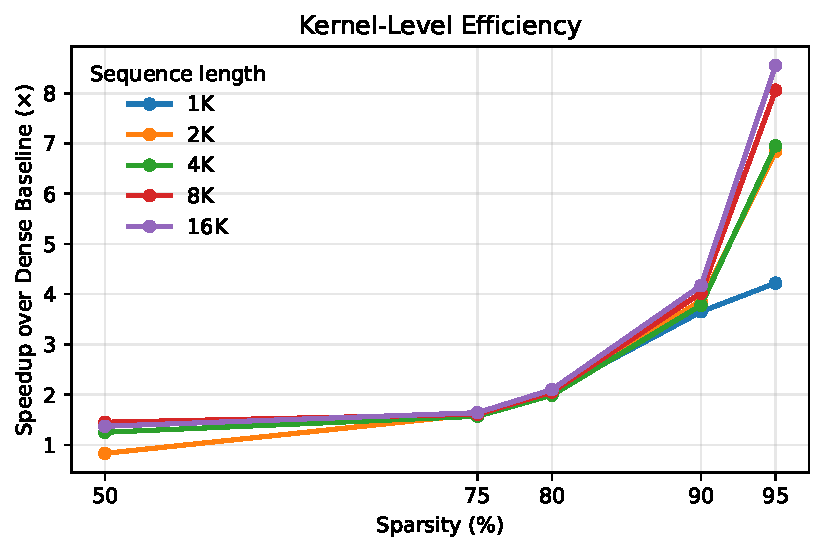
\includegraphics[width=1\linewidth]{figures/kernel_speedup.pdf}
    \caption{Kernel-level wall-clock speedup of the fused block-sparse attention kernel over the dense Flash Attention baseline. Speedup increases with both sequence length and sparsity ratio, reaching $8.6\times$ at 16K tokens with 95\% sparsity.}
    \label{fig:kernel}
\end{figure}

\subsection{Ablation Studies}

We next isolate the two design choices that distinguish Step-dLLM from SparseD: periodic mask refreshing and head-adaptive budget allocation. Unless otherwise specified, all ablations are conducted on LLaDA-1.5 with block size 16.

\paragraph{Refresh frequency.}
Table~\ref{tab:ablation-freq} shows that refresh frequency is a first-order factor. As the refresh interval becomes shorter, both SparseD and Step-dLLM improve, but the gain is consistently larger for Step-dLLM. On GSM8K at 90\% sparsity, SparseD improves from 29.64\% to 43.90\% when moving from one-shot masking ($f{=}1.0$) to frequent refresh ($f{=}0.2$), whereas Step-dLLM improves from 35.18\% to 61.79\%. This confirms that cross-step mask reuse should be local rather than global.

\paragraph{Head-adaptive budget.}
The head-adaptive allocation also contributes independently of refresh. Even under the same one-shot setting ($f{=}1.0$), Step-dLLM still outperforms SparseD, indicating that a better allocation of sparse budget across heads leads to a better mask even before refresh is introduced. For example, Step-dLLM improves GSM8K from 29.64\% to 35.18\% at 90\% sparsity and improves RULER-VT from 86.16\% to 92.32\% at 95\% sparsity. This supports the intuition that different heads exhibit different concentration patterns and should not be forced to share a uniform sparsity rule.

\paragraph{Block size.}
Finally, Table~\ref{tab:ablation-blocksize} shows that Step-dLLM remains stronger than SparseD at both block sizes 16 and 32, and its advantage becomes larger with coarser blocks. At 90\% sparsity on GSM8K, the margin grows from 5.6 points at block size 16 to 22.0 points at block size 32. This trend is expected: when each masking decision removes a larger block, stale masks become more costly, so step-aware refresh and adaptive budget allocation matter even more.

\begin{table}[t]
\centering
\caption{Ablation on mask refresh frequency (LLaDA-1.5, block size 16). Frequency $f$ means the mask is refreshed every $f \times N_{\text{steps}}$ steps; lower $f$ corresponds to more frequent updates. All values are accuracy (\%). \textbf{Bold} marks the best per sparsity level.}
\label{tab:ablation-freq}
\setlength{\tabcolsep}{5pt}
\renewcommand{\arraystretch}{1.15}

\resizebox{\textwidth}{!}{%
\begin{tabular}{@{}ll cccc cccc@{}}
\toprule
\multirow{2.5}{*}{\textbf{Sparsity}} & \multirow{2.5}{*}{\textbf{Metric}}
  & \multicolumn{4}{c}{\textbf{SparseD}}
  & \multicolumn{4}{c}{\textbf{Step-dLLM}} \\
\cmidrule(lr){3-6} \cmidrule(l){7-10}
& & $f{=}1.0$ & $f{=}0.5$ & $f{=}0.3$ & $f{=}0.2$
  & $f{=}1.0$ & $f{=}0.5$ & $f{=}0.3$ & $f{=}0.2$ \\
\midrule

\multirow{3}{*}{95\%}
  & GSM8K    &  9.48 &  6.29 &  5.53 &  6.29 & 16.83 & 16.98 & 17.43 & \textbf{18.80} \\
  & MATH     & 12.00 & 13.80 & 14.20 & 13.60 & 15.40 & 16.00 & 15.40 & \textbf{16.60} \\
  & RULER-VT & 86.16 & 95.40 & 97.04 & 96.64 & 92.32 & 95.36 & 96.36 & \textbf{97.20} \\

\midrule
\multirow{3}{*}{90\%}
  & GSM8K    & 29.64 & 29.72 & 34.19 & 43.90 & 35.18 & 40.64 & 52.24 & \textbf{61.79} \\
  & MATH     & 23.00 & 22.20 & 23.20 & 24.80 & 21.20 & 22.60 & 23.60 & \textbf{26.20} \\
  & RULER-VT & 93.64 & 97.04 & 97.96 & 97.96 & 94.00 & 96.56 & 97.04 & \textbf{97.50} \\

\midrule
\multirow{3}{*}{80\%}
  & GSM8K    & 53.68 & 64.37 & 73.09 & 76.80 & 57.77 & 68.23 & 75.01 & \textbf{77.56} \\
  & MATH     & 29.20 & 31.20 & 32.40 & 34.00 & 31.00 & 32.00 & 33.60 & \textbf{36.40} \\
  & RULER-VT & 94.32 &    -- &    -- &    -- & 98.52 & 96.64 & 97.28 & \textbf{99.88} \\

\bottomrule
\end{tabular}%
}
\end{table}

\begin{table}[t]
\centering
\caption{Ablation on block size (LLaDA-1.5). Accuracy (\%) on short-form benchmarks under block sizes 16 and 32. Step-dLLM consistently outperforms SparseD at both granularities. \textbf{Bold} marks the best per row.}
\label{tab:ablation-blocksize}
\small
\setlength{\tabcolsep}{5pt}
\renewcommand{\arraystretch}{1.12}

\begin{tabular}{llcccc}
\toprule
\multirow{2}{*}{Sparsity} & \multirow{2}{*}{Benchmark}
& \multicolumn{2}{c}{Block size = 16} & \multicolumn{2}{c}{Block size = 32} \\
\cmidrule(lr){3-4} \cmidrule(lr){5-6}
& & SparseD & Step-dLLM & SparseD & Step-dLLM \\
\midrule

\multirow{3}{*}{95\%}
& GSM8K     &  9.86 & \textbf{17.13} &  8.64 & \textbf{19.18} \\
& MATH      &  9.40 & \textbf{13.80} & 10.60 & \textbf{16.20} \\
& HumanEval & 20.12 & \textbf{21.34} & 12.80 & \textbf{23.78} \\
\midrule

\multirow{3}{*}{90\%}
& GSM8K     & 29.64 & \textbf{35.25} & 17.51 & \textbf{39.50} \\
& MATH      & \textbf{20.00} & \textbf{21.60} & 21.60 & \textbf{26.00} \\
& HumanEval & 30.49 & \textbf{32.93} & 28.66 & \textbf{34.15} \\
\midrule

\multirow{3}{*}{80\%}
& GSM8K     & 53.68 & \textbf{58.38} & 50.87 & \textbf{63.23} \\
& MATH      & \textbf{28.20} & 27.60 & 31.60 & 31.20 \\
& HumanEval & 36.59 & \textbf{37.20} & 37.80 & \textbf{39.12} \\

\bottomrule
\end{tabular}
\end{table}



% \subsection{Main Results}
% %We present the inference accuracy of Step-dLLM and all baselines on Llada-1.5 and Dream-7B across all benchmarks, as shown in Table 1.
% We evaluate Step-dLLM on two representative diffusion LLMs, LlaDA-1.5 and Dream-7B-Instruct (Table~\ref{tab:main-bs16-llada} and Table~\ref{tab:main-bs16-dream}), covering short-form reasoning/code benchmarks (GSM8K, MATH, HumanEval) and long-context benchmarks (NIAH, RULER). All methods are compared under the same sparsity budgets (50\% 80\% 90\% 95\%) against Dense, StreamingLLM, and SparseD. Overall, StreamingLLM exhibits a severe quality collapse on diffusion LLMs, while Step-dLLM is consistently more robust—especially at high sparsity (90\%–95\%)—and preserves strong long-context performance, validating the benefit of step-aware sparse updates and global budget allocation under denoising-step dynamics.

% Table~\ref{tab:main-bs16-llada} and Table~\ref{tab:main-bs16-dream} show that Step-dLLM is consistently more robust than SparseD at high sparsity(90\%–95\%) on both LlaDA-1.5 and Dream-7B-Instruct, because it aligns the sparsity pattern with DLLMs step dynamics: unlike SparseD’s largely step-agnostic masking, Step-dLLM leverages the fact that attention-score structure is correlated across denoising steps but shifts across stages, so it reuses masks when cross-step similarity is high and refreshes them when the step/stage distribution changes. This step-aware, stage-aware mask updating prevents the “stale mask” failure mode under aggressive sparsity, thereby preserving reasoning/code accuracy while maintaining long-context quality on NIAH/RULER.

% Also, the tables demonstrate that Step-dLLM delivers a better accuracy–efficiency tradeoff than SparseD at high sparsity (90\%–95\%) and avoids the quality collapse of traditional AR mathod, like StreamingLLM, on DLLMs.


% Model: LLaDA-1.5, Dream-7B-Instruct

% Bench: MATH500, Human-eval, RULER, NIAH, GSM8K

% Baseline: StreamingLLM, SparseD, FastDLLM

% \begin{itemize}
% \item Dense
% \item + StreamingLLM
% \item + SparseD
% % \item + OPT1
% \item + Ours
% \item (optional) fastdllm
% \end{itemize}

% Setting:
% Sparsity: 95\%, 90\%, 80\%, 50\%

% Step updating: 1/2, 1/3, 1/5, 1/10, 0

% Block Size: 16, 32

% \begin{table}[t]
\centering
\caption{Main results on LLaDA-1.5 with block size 16. All values are accuracy (\%). \textbf{Bold} marks the best result per sparsity level (excluding Dense).}
\label{tab:main-bs16-llada}
\setlength{\tabcolsep}{3.5pt}
\renewcommand{\arraystretch}{1.15}

\resizebox{\textwidth}{!}{%
\begin{tabular}{@{}ll ccc ccccccccc ccccc@{}}
\toprule
\multirow{2.5}{*}{\textbf{Method}} & \multirow{2.5}{*}{\textbf{Sparsity}}
  & \multicolumn{3}{c}{\textbf{Short-form}}
  & \multicolumn{8}{c}{\textbf{NIAH}}
  & \multicolumn{5}{c}{\textbf{RULER}} \\
\cmidrule(lr){3-5} \cmidrule(lr){6-13} \cmidrule(l){14-18}
& & GSM8K & Math & HumanE
  & $\text{S}_1$ & $\text{S}_2$ & $\text{S}_3$
  & $\text{MK}_1$ & $\text{MK}_2$ & $\text{MK}_3$
  & MQ & MV
  & VT & CWE & FWE & QS & QH \\
\midrule

Dense & --
  & \textbf{81.04} & \textbf{37.20} & \textbf{40.24}
  & \textbf{100.0} & \textbf{100.0} & \textbf{100.0} & \textbf{100.0}
  & \textbf{100.0} & \textbf{100.0} & \textbf{100.0} & \textbf{100.0}
  & \textbf{100.0} & \textbf{52.40} & \textbf{64.20} & \textbf{91.30} & \textbf{76.00} \\

\midrule
\multirow{3}{*}{StreamingLLM}
  & 50\% & 74.07 & \textbf{38.20} & 39.02
    & 20.80 & 20.20 & 18.40 & 21.20 & 20.40 & 15.40 & 19.20 & 14.40
    & 30.60 & 13.40 & 73.80 & 81.65 & 44.40 \\
  & 80\% & 19.11 & 13.60 & 19.51
    & 5.00 & 2.40 & 1.40 & 3.40 & 3.60 & 0.00 & 2.10 & 2.10
    & 6.56 & 3.02 & 76.27 & 20.48 & 22.40 \\
  & 90\% & 0.08 & 0.00 & 2.43
    & 0.00 & 0.00 & 0.00 & 0.00 & 0.00 & 0.00 & 0.00 & 0.00
    & 0.00 & 2.12 & 0.00 & 0.27 & 0.00 \\

\midrule
\multirow{4}{*}{SparseD}
  & 50\% & 80.59 & 37.40 & 42.68
    & \textbf{100.0} & \textbf{100.0} & \textbf{100.0} & \textbf{100.0}
    & \textbf{100.0} & \textbf{100.0} & \textbf{100.0} & \textbf{100.0}
    & \textbf{99.88} & 52.26 & \textbf{61.40} & \textbf{83.17} & 77.60 \\
  & 80\% & 53.68 & \textbf{28.20} & 36.59
    & \textbf{100.0} & \textbf{100.0} & 71.20 & \textbf{100.0}
    & \textbf{100.0} & 74.20 & 85.85 & 79.10
    & 94.28 & \textbf{57.80} & 45.40 & 83.48 & 77.80 \\
  & 90\% & 29.64 & 20.00 & 30.49
    & \textbf{100.0} & \textbf{100.0} & 76.60 & \textbf{100.0}
    & 99.80 & 77.20 & 82.85 & 80.60
    & 93.32 & 34.56 & 42.07 & 83.13 & 76.00 \\
  & 95\% & 9.86 & 9.40 & 20.12
    & \textbf{100.0} & \textbf{100.0} & 79.40 & \textbf{100.0}
    & \textbf{100.0} & 78.20 & 81.80 & 81.10
    & 86.64 & 39.92 & 39.00 & \textbf{81.97} & \textbf{73.60} \\

\midrule
\multirow{4}{*}{\textbf{Step-dLLM}}
  & 50\% & \textbf{82.71} & 36.80 & \textbf{42.68}
    & \textbf{100.0} & \textbf{100.0} & \textbf{100.0} & \textbf{100.0}
    & \textbf{100.0} & \textbf{100.0} & \textbf{100.0} & \textbf{100.0}
    & 99.60 & \textbf{53.16} & 60.87 & 83.03 & \textbf{78.60} \\
  & 80\% & \textbf{58.38} & 27.60 & \textbf{37.20}
    & \textbf{100.0} & \textbf{100.0} & \textbf{100.0} & \textbf{100.0}
    & 99.80 & \textbf{99.60} & \textbf{99.90} & \textbf{98.60}
    & \textbf{98.52} & 56.46 & \textbf{51.73} & \textbf{83.73} & \textbf{78.20} \\
  & 90\% & \textbf{35.25} & \textbf{21.60} & \textbf{32.93}
    & \textbf{100.0} & \textbf{100.0} & \textbf{100.0} & \textbf{100.0}
    & \textbf{100.0} & \textbf{97.60} & \textbf{99.65} & \textbf{95.90}
    & \textbf{94.00} & \textbf{54.16} & \textbf{46.80} & \textbf{83.48} & \textbf{76.40} \\
  & 95\% & \textbf{17.13} & \textbf{13.80} & \textbf{21.34}
    & \textbf{100.0} & \textbf{100.0} & \textbf{98.80} & \textbf{100.0}
    & \textbf{100.0} & \textbf{88.40} & \textbf{95.25} & \textbf{92.30}
    & \textbf{92.32} & \textbf{44.76} & \textbf{44.07} & 81.37 & 71.40 \\
\bottomrule
\end{tabular}%
}
\end{table}

% \begin{table}[t]
\centering
\caption{Main results on Dream-7B-Instruct with block size 16. All values are accuracy (\%). \textbf{Bold} marks the best result per sparsity level (excluding Dense).}
\label{tab:main-bs16-dream}
\setlength{\tabcolsep}{3.5pt}
\renewcommand{\arraystretch}{1.15}

\resizebox{\textwidth}{!}{%
\begin{tabular}{@{}ll ccc ccccccccc ccccc@{}}
\toprule
\multirow{2.5}{*}{\textbf{Method}} & \multirow{2.5}{*}{\textbf{Sparsity}}
  & \multicolumn{3}{c}{\textbf{Short-form}}
  & \multicolumn{8}{c}{\textbf{NIAH}}
  & \multicolumn{5}{c}{\textbf{RULER}} \\
\cmidrule(lr){3-5} \cmidrule(lr){6-13} \cmidrule(l){14-18}
& & GSM8K & Math & HumanE
  & $\text{S}_1$ & $\text{S}_2$ & $\text{S}_3$
  & $\text{MK}_1$ & $\text{MK}_2$ & $\text{MK}_3$
  & MQ & MV
  & VT & CWE & FWE & QS & QH \\
\midrule

Dense & --
  & \textbf{77.41} & \textbf{45.60} & --
  & \textbf{100.0} & \textbf{100.0} & \textbf{91.00} & \textbf{98.00}
  & \textbf{99.80} & \textbf{77.60} & \textbf{97.70} & \textbf{96.40}
  & \textbf{96.32} & \textbf{87.28} & \textbf{79.47} & \textbf{79.57} & \textbf{64.00} \\

\midrule
\multirow{3}{*}{StreamingLLM}
  & 50\% & 38.13 & 8.80 & 42.70
    & 10.00 & 11.00 & 9.00 & 11.00 & 8.80 & 12.40 & 8.75 & 10.30
    & 13.40 & 43.34 & 37.73 & \textbf{81.40} & 33.00 \\
  & 80\% & 19.56 & 10.40 & 25.00
    & 1.80 & 2.80 & 1.40 & 3.20 & 1.20 & 0.00 & 1.95 & 2.40
    & 0.36 & 4.54 & 4.33 & 19.18 & 19.60 \\
  & 90\% & 0.00 & 0.00 & 2.44
    & 0.00 & 0.00 & 0.00 & 0.00 & 0.00 & 0.00 & 0.00 & 0.00
    & 0.00 & 0.00 & 0.00 & 0.00 & 0.00 \\

\midrule
\multirow{4}{*}{SparseD}
  & 50\% & 70.50 & 43.60 & 56.10
    & \textbf{100.0} & \textbf{100.0} & 90.20 & \textbf{98.00} & 99.40 & \textbf{75.80}
    & \textbf{97.45} & 97.40
    & 96.28 & \textbf{85.16} & \textbf{75.80} & 80.37 & \textbf{64.60} \\
  & 80\% & 49.81 & 37.80 & 53.66
    & \textbf{100.0} & \textbf{99.80} & 47.20 & \textbf{98.80} & \textbf{99.80} & 46.80
    & 60.05 & 69.30
    & 95.44 & 71.76 & \textbf{71.77} & \textbf{79.50} & 61.00 \\
  & 90\% & 22.21 & 28.80 & 43.90
    & \textbf{100.0} & \textbf{100.0} & 44.60 & \textbf{98.80} & \textbf{99.80} & \textbf{44.80}
    & \textbf{59.45} & \textbf{69.00}
    & 92.20 & 54.72 & 67.53 & 78.45 & \textbf{61.60} \\
  & 95\% & 4.40 & 14.80 & 31.10
    & \textbf{100.0} & \textbf{100.0} & \textbf{40.80} & \textbf{98.40} & 99.40 & \textbf{37.40}
    & \textbf{53.95} & \textbf{66.85}
    & 78.64 & 43.84 & 62.26 & 77.60 & 60.00 \\

\midrule
\multirow{4}{*}{\textbf{Step-dLLM}}
  & 50\% & \textbf{71.80} & \textbf{44.00} & \textbf{58.54}
    & \textbf{100.0} & \textbf{100.0} & \textbf{90.50} & 97.80 & \textbf{99.80} & 75.60
    & 97.25 & \textbf{97.50}
    & \textbf{96.40} & 83.24 & 75.53 & 79.80 & 63.80 \\
  & 80\% & \textbf{52.39} & \textbf{38.60} & \textbf{54.27}
    & \textbf{100.0} & \textbf{99.80} & \textbf{69.00} & 98.20 & \textbf{99.80} & \textbf{65.40}
    & \textbf{74.10} & \textbf{78.40}
    & \textbf{96.04} & \textbf{73.24} & 71.13 & 78.53 & \textbf{61.80} \\
  & 90\% & \textbf{32.68} & \textbf{32.00} & \textbf{50.00}
    & \textbf{100.0} & 99.80 & \textbf{47.00} & 97.20 & \textbf{99.80} & 39.80
    & 57.30 & 68.05
    & \textbf{94.68} & \textbf{59.58} & \textbf{68.26} & \textbf{79.03} & 60.20 \\
  & 95\% & \textbf{15.31} & \textbf{19.20} & \textbf{35.98}
    & \textbf{100.0} & 99.60 & 37.20 & 95.60 & \textbf{99.60} & 33.60
    & 52.30 & 60.95
    & \textbf{82.08} & \textbf{46.90} & \textbf{62.87} & \textbf{77.83} & \textbf{61.40} \\
\bottomrule
\end{tabular}%
}
\end{table}

% %\begin{table}[t]
\centering
\caption{Long-context results on LLaDA-1.5 with block size 16 (NIAH and RULER benchmarks). All values are accuracy (\%). \textbf{Bold} marks the best result per sparsity level (excluding Dense).}
\label{tab:main-bs16-llada-long}
\setlength{\tabcolsep}{3.5pt}
\renewcommand{\arraystretch}{1.15}

\resizebox{\textwidth}{!}{%
\begin{tabular}{@{}ll cccccccc ccccc@{}}
\toprule
\multirow{2.5}{*}{\textbf{Method}} & \multirow{2.5}{*}{\textbf{Sparsity}}
  & \multicolumn{8}{c}{\textbf{NIAH}}
  & \multicolumn{5}{c}{\textbf{RULER}} \\
\cmidrule(lr){3-10} \cmidrule(l){11-15}
& & $\text{S}_1$ & $\text{S}_2$ & $\text{S}_3$
  & $\text{MK}_1$ & $\text{MK}_2$ & $\text{MK}_3$
  & MQ & MV
  & VT & CWE & FWE & QS & QH \\
\midrule

Dense & --
  & \textbf{100.0} & \textbf{100.0} & \textbf{100.0} & \textbf{100.0}
  & \textbf{100.0} & \textbf{100.0} & \textbf{100.0} & \textbf{100.0}
  & \textbf{100.0} & \textbf{52.40} & \textbf{64.20} & \textbf{91.30} & \textbf{76.00} \\

\midrule
\multirow{3}{*}{StreamingLLM}
  & 50\% & 20.80 & 20.20 & 18.40 & 21.20 & 20.40 & 15.40 & 19.20 & 14.40
    & 30.60 & 13.40 & 73.80 & 81.65 & 44.40 \\
  & 80\% & 5.00 & 2.40 & 1.40 & 3.40 & 3.60 & 0.00 & 2.10 & 2.10
    & 6.56 & 3.02 & 76.27 & 20.48 & 22.40 \\
  & 90\% & 0.00 & 0.00 & 0.00 & 0.00 & 0.00 & 0.00 & 0.00 & 0.00
    & 0.00 & 2.12 & 0.00 & 0.27 & 0.00 \\

\midrule
\multirow{4}{*}{SparseD}
  & 50\% & \textbf{100.0} & \textbf{100.0} & \textbf{100.0} & \textbf{100.0}
    & \textbf{100.0} & \textbf{100.0} & \textbf{100.0} & \textbf{100.0}
    & \textbf{99.88} & 52.26 & \textbf{61.40} & \textbf{83.17} & 77.60 \\
  & 80\% & \textbf{100.0} & \textbf{100.0} & 71.20 & \textbf{100.0}
    & \textbf{100.0} & 74.20 & 85.85 & 79.10
    & 94.28 & \textbf{57.80} & 45.40 & 83.48 & 77.80 \\
  & 90\% & \textbf{100.0} & \textbf{100.0} & 76.60 & \textbf{100.0}
    & 99.80 & 77.20 & 82.85 & 80.60
    & 93.32 & 34.56 & 42.07 & 83.13 & 76.00 \\
  & 95\% & \textbf{100.0} & \textbf{100.0} & 79.40 & \textbf{100.0}
    & \textbf{100.0} & 78.20 & 81.80 & 81.10
    & 86.64 & 39.92 & 39.00 & \textbf{81.97} & \textbf{73.60} \\

\midrule
\multirow{4}{*}{\textbf{Step-dLLM}}
  & 50\% & \textbf{100.0} & \textbf{100.0} & \textbf{100.0} & \textbf{100.0}
    & \textbf{100.0} & \textbf{100.0} & \textbf{100.0} & \textbf{100.0}
    & 99.60 & \textbf{53.16} & 60.87 & 83.03 & \textbf{78.60} \\
  & 80\% & \textbf{100.0} & \textbf{100.0} & \textbf{100.0} & \textbf{100.0}
    & 99.80 & \textbf{99.60} & \textbf{99.90} & \textbf{98.60}
    & \textbf{98.52} & 56.46 & \textbf{51.73} & \textbf{83.73} & \textbf{78.20} \\
  & 90\% & \textbf{100.0} & \textbf{100.0} & \textbf{100.0} & \textbf{100.0}
    & \textbf{100.0} & \textbf{97.60} & \textbf{99.65} & \textbf{95.90}
    & \textbf{94.00} & \textbf{54.16} & \textbf{46.80} & \textbf{83.48} & \textbf{76.40} \\
  & 95\% & \textbf{100.0} & \textbf{100.0} & \textbf{98.80} & \textbf{100.0}
    & \textbf{100.0} & \textbf{88.40} & \textbf{95.25} & \textbf{92.30}
    & \textbf{92.32} & \textbf{44.76} & \textbf{44.07} & 81.37 & 71.40 \\
\bottomrule
\end{tabular}%
}
\end{table}





% % \subsection{Efficiency}
% Sequence length (total): 1K, 2K, 4K (@JUNPAN)

% Kernel-level: all heads block-wise sparse attention

% e2e: + step-update + sparse attn

% Figure~\ref{fig:kernel}
% \begin{figure}[t]
%     \centering
%     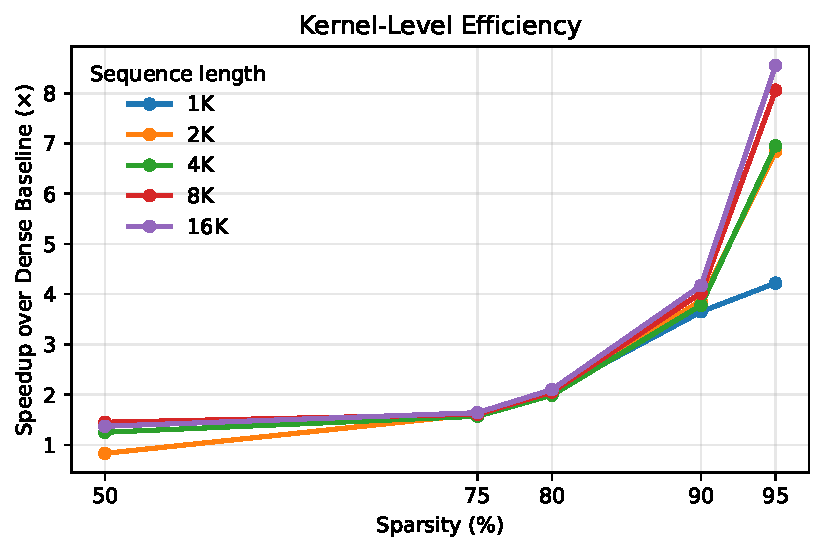
\includegraphics[width=1\linewidth]{figures/kernel_speedup.pdf}
%     \caption{Kernel-level speedup over the dense baseline under different sparsity levels and sequence lengths. Larger gains are achieved in longer-context and higher-sparsity regimes.}
%     \label{fig:kernel}
% \end{figure}
% summarizes the kernel-level efficiency of our Step-dLLM implementation. Specifically, we develop a customized CUDA kernel that fuses step-aware mask updating with block-wise sparse attention, and benchmark its end-to-end runtime under different sequence lengths (from 1K to 16K) and sparsity budgets. Across all settings, the proposed kernel achieves substantial speedups over the dense baseline, with gains increasing as either the sequence length grows or the sparsity becomes more aggressive, reaching up to ~8× speedup at long-context and high-sparsity regimes. This shows that Step-dLLM’s step-aware sparse attention is not only algorithmically effective but also practically efficient at the kernel level.

% %\begin{table}[H]
  \centering
  \caption{Add caption}
  \label{tab:main-kernel-level}

  \small
  \setlength{\tabcolsep}{4pt}
  \renewcommand{\arraystretch}{1.08}

  \resizebox{\columnwidth}{!}{%
    \begin{tabular}{ccccc}
    \toprule
    Kernel Size & Sparsity & Baseline (dense) & Ours & Speedup \\
    \midrule

    \multirow{5}{*}{1K}
      & 95\% & 0.053041 & 0.01257000 & 4.22 \\
      & 90\% & 0.053041 & 0.01452900 & 3.65 \\
      & 80\% & 0.053041 & 0.02579500 & 2.06 \\
      & 75\% & 0.053041 & 0.03299900 & 1.61 \\
      & 50\% & 0.053041 & 0.06417000 & 0.83 \\
    \midrule

    \multirow{5}{*}{2K}
      & 95\% & 0.193364 & 0.02827213 & 6.84 \\
      & 90\% & 0.193364 & 0.04997750 & 3.87 \\
      & 80\% & 0.193364 & 0.09559138 & 2.02 \\
      & 75\% & 0.193364 & 0.12004263 & 1.61 \\
      & 50\% & 0.193364 & 0.23373875 & 0.83 \\
    \midrule

    \multirow{5}{*}{4K}
      & 95\% & 0.763358 & 0.10975700 & 6.95 \\
      & 90\% & 0.763358 & 0.20190700 & 3.78 \\
      & 80\% & 0.763358 & 0.38442200 & 1.99 \\
      & 75\% & 0.763358 & 0.48581000 & 1.57 \\
      & 50\% & 0.763358 & 0.61274000 & 1.25 \\
    \midrule

    \multirow{5}{*}{8K}
      & 95\% & 2.952540 & 0.36623300 & 8.06 \\
      & 90\% & 2.952540 & 0.73515000 & 4.02 \\
      & 80\% & 2.952540 & 1.43898800 & 2.05 \\
      & 75\% & 2.952540 & 1.83316500 & 1.61 \\
      & 50\% & 2.952540 & 2.03316500 & 1.45 \\
    \midrule

    \multirow{5}{*}{16K}
      & 95\% & 11.837924 & 1.38469300 & 8.55 \\
      & 90\% & 11.837924 & 2.84201000 & 4.17 \\
      & 80\% & 11.837924 & 5.63847300 & 2.10 \\
      & 75\% & 11.837924 & 7.21230000 & 1.64 \\
      & 50\% & 11.837924 & 8.61280000 & 1.37 \\
    \bottomrule
    \end{tabular}%
  }
\end{table}

% \subsection{Ablation Study}

% 1. Block size: 8, 16, 32

% We also did further ablation study for block size 32, since the StreamingLLM doesn't have block size, we only compare the results of SparseD and Ours. The results of experimention are shown in table 4 & table 5:

% %\begin{table}[t]
\centering
\caption{Main results on LLaDA-1.5 with block size 32. All values are accuracy (\%). \textbf{Bold} marks the best result per sparsity level (excluding Dense).}
\label{tab:main-bs32-llada}
\setlength{\tabcolsep}{3.5pt}
\renewcommand{\arraystretch}{1.15}

\resizebox{\textwidth}{!}{%
\begin{tabular}{@{}ll ccc ccccccccc ccccc@{}}
\toprule
\multirow{2.5}{*}{\textbf{Method}} & \multirow{2.5}{*}{\textbf{Sparsity}}
  & \multicolumn{3}{c}{\textbf{Short-form}}
  & \multicolumn{8}{c}{\textbf{NIAH}}
  & \multicolumn{5}{c}{\textbf{RULER}} \\
\cmidrule(lr){3-5} \cmidrule(lr){6-13} \cmidrule(l){14-18}
& & GSM8K & Math & HumanE
  & $\text{S}_1$ & $\text{S}_2$ & $\text{S}_3$
  & $\text{MK}_1$ & $\text{MK}_2$ & $\text{MK}_3$
  & MQ & MV
  & VT & CWE & FWE & QS & QH \\
\midrule

Dense & --
  & \textbf{81.04} & \textbf{37.20} & \textbf{40.24}
  & \textbf{100.0} & \textbf{100.0} & \textbf{100.0} & \textbf{100.0}
  & \textbf{100.0} & \textbf{100.0} & \textbf{100.0} & \textbf{100.0}
  & \textbf{100.0} & \textbf{52.40} & \textbf{64.20} & \textbf{91.30} & \textbf{76.00} \\

\midrule
\multirow{4}{*}{SparseD}
  & 50\% & \textbf{73.09} & \textbf{40.60} & 40.85
    & \textbf{100.0} & \textbf{100.0} & \textbf{100.0} & \textbf{100.0}
    & \textbf{100.0} & \textbf{100.0} & -- & --
    & \textbf{100.0} & 49.00 & \textbf{66.93} & \textbf{83.43} & 77.40 \\
  & 80\% & 46.17 & \textbf{31.60} & 37.80
    & \textbf{100.0} & \textbf{100.0} & 87.60 & \textbf{100.0}
    & \textbf{100.0} & 93.60 & -- & --
    & 99.56 & 48.26 & 52.73 & \textbf{83.77} & 77.00 \\
  & 90\% & 17.29 & 21.60 & 28.66
    & \textbf{100.0} & \textbf{100.0} & 88.00 & \textbf{100.0}
    & \textbf{100.0} & 94.00 & 98.00 & 90.80
    & 93.32 & 46.64 & 49.93 & \textbf{84.23} & 75.40 \\
  & 95\% & 12.66 & 10.60 & 12.80
    & \textbf{100.0} & \textbf{100.0} & \textbf{88.20} & \textbf{100.0}
    & \textbf{100.0} & 92.80 & \textbf{98.55} & 88.80
    & 63.00 & 43.44 & 30.80 & 83.45 & 73.60 \\

\midrule
\multirow{4}{*}{\textbf{Step-dLLM}}
  & 50\% & \textbf{73.09} & 40.40 & \textbf{42.07}
    & \textbf{100.0} & \textbf{100.0} & \textbf{100.0} & \textbf{100.0}
    & \textbf{100.0} & \textbf{100.0} & -- & --
    & 99.92 & \textbf{49.14} & 63.07 & 82.50 & \textbf{77.60} \\
  & 80\% & \textbf{57.39} & 31.20 & \textbf{39.12}
    & \textbf{100.0} & \textbf{100.0} & \textbf{94.80} & \textbf{100.0}
    & \textbf{100.0} & \textbf{96.80} & -- & --
    & \textbf{99.80} & \textbf{51.28} & \textbf{57.00} & 83.23 & \textbf{77.20} \\
  & 90\% & \textbf{40.86} & \textbf{26.00} & \textbf{34.15}
    & \textbf{100.0} & \textbf{100.0} & \textbf{88.20} & \textbf{100.0}
    & \textbf{100.0} & \textbf{95.40} & \textbf{98.60} & \textbf{93.65}
    & \textbf{98.48} & \textbf{50.02} & \textbf{50.13} & 82.37 & \textbf{76.40} \\
  & 95\% & \textbf{21.60} & \textbf{16.20} & \textbf{23.78}
    & \textbf{100.0} & \textbf{100.0} & 87.80 & \textbf{100.0}
    & \textbf{100.0} & \textbf{94.00} & 98.50 & \textbf{91.00}
    & \textbf{89.28} & \textbf{47.24} & \textbf{44.67} & \textbf{83.53} & \textbf{74.80} \\
\bottomrule
\end{tabular}%
}
\end{table}

% %\begin{table}[t]
\centering
\caption{Main results on Dream-7B-Instruct with block size 32. All values are accuracy (\%). \textbf{Bold} marks the best result per sparsity level (excluding Dense).}
\label{tab:main-bs32-dream}
\setlength{\tabcolsep}{3.5pt}
\renewcommand{\arraystretch}{1.15}

\resizebox{\textwidth}{!}{%
\begin{tabular}{@{}ll ccc ccccccccc ccccc@{}}
\toprule
\multirow{2.5}{*}{\textbf{Method}} & \multirow{2.5}{*}{\textbf{Sparsity}}
  & \multicolumn{3}{c}{\textbf{Short-form}}
  & \multicolumn{8}{c}{\textbf{NIAH}}
  & \multicolumn{5}{c}{\textbf{RULER}} \\
\cmidrule(lr){3-5} \cmidrule(lr){6-13} \cmidrule(l){14-18}
& & GSM8K & Math & HumanE
  & $\text{S}_1$ & $\text{S}_2$ & $\text{S}_3$
  & $\text{MK}_1$ & $\text{MK}_2$ & $\text{MK}_3$
  & MQ & MV
  & VT & CWE & FWE & QS & QH \\
\midrule

Dense & --
  & \textbf{77.41} & \textbf{45.60} & --$^\dagger$
  & \textbf{100.0} & \textbf{100.0} & \textbf{91.00} & \textbf{98.00}
  & \textbf{99.80} & \textbf{77.60} & \textbf{97.70} & \textbf{96.40}
  & \textbf{96.32} & \textbf{87.28} & \textbf{79.47} & \textbf{79.57} & \textbf{64.00} \\

\midrule
\multirow{4}{*}{SparseD}
  & 50\% & \textbf{73.09} & 42.00 & 56.10
    & \textbf{100.0} & 99.80 & 92.40 & \textbf{98.40} & \textbf{99.80} & 76.00
    & \textbf{97.55} & \textbf{98.05}
    & 96.20 & \textbf{84.48} & \textbf{76.40} & 79.73 & \textbf{64.00} \\
  & 80\% & 46.17 & 39.20 & 53.05
    & \textbf{100.0} & \textbf{99.80} & 75.00 & \textbf{98.60} & \textbf{99.80} & 70.60
    & 90.70 & 97.75
    & 94.12 & 68.64 & 72.07 & \textbf{80.57} & \textbf{64.60} \\
  & 90\% & 17.29 & 29.20 & \textbf{49.39}
    & \textbf{100.0} & \textbf{99.80} & \textbf{72.60} & \textbf{98.00} & \textbf{99.80} & 68.80
    & \textbf{89.80} & \textbf{96.95}
    & 80.60 & 53.80 & 67.87 & \textbf{79.40} & \textbf{64.40} \\
  & 95\% & 12.66 & 11.60 & 21.34
    & \textbf{100.0} & \textbf{97.80} & \textbf{70.20} & \textbf{90.20} & 99.40 & 64.20
    & \textbf{78.95} & \textbf{81.85}
    & \textbf{24.52} & 44.38 & \textbf{62.60} & 77.87 & \textbf{60.60} \\

\midrule
\multirow{4}{*}{\textbf{Step-dLLM}}
  & 50\% & \textbf{73.09} & \textbf{44.60} & \textbf{58.54}
    & \textbf{100.0} & \textbf{100.0} & \textbf{93.20} & \textbf{98.40} & \textbf{99.80} & \textbf{77.20}
    & 96.00 & 97.95
    & \textbf{96.52} & 83.28 & 76.13 & \textbf{80.18} & 63.80 \\
  & 80\% & \textbf{57.39} & \textbf{39.80} & \textbf{53.66}
    & \textbf{100.0} & \textbf{99.80} & \textbf{75.60} & 98.20 & \textbf{99.80} & \textbf{71.20}
    & \textbf{90.85} & \textbf{98.25}
    & \textbf{95.76} & \textbf{72.10} & \textbf{72.20} & 79.17 & 63.20 \\
  & 90\% & \textbf{40.86} & \textbf{30.60} & 47.56
    & \textbf{100.0} & \textbf{99.80} & 72.20 & 94.60 & \textbf{99.80} & \textbf{70.00}
    & 88.15 & 96.25
    & \textbf{91.56} & \textbf{59.36} & \textbf{69.60} & 78.67 & 63.00 \\
  & 95\% & \textbf{21.60} & \textbf{20.40} & \textbf{33.54}
    & \textbf{100.0} & 86.80 & 67.40 & 83.60 & \textbf{99.60} & \textbf{67.60}
    & 74.10 & 74.40
    & 20.40 & \textbf{47.07} & 59.93 & 75.77 & \textbf{60.60} \\
\bottomrule
\multicolumn{18}{@{}l}{\footnotesize $^\dagger$\,HumanEval not evaluated for Dream-7B-Instruct under dense inference.}
\end{tabular}%
}
\end{table}


% 2. Step update frequency: 

% 3. OPT1, OPT2

% 4. Accuracy \& efficiency tradeoff

